\documentclass[10pt, twocolumn]{article}

\usepackage{graphicx}
\usepackage{color}
\usepackage[margin=1in]{geometry}
\usepackage{enumitem}
\usepackage{bbding}
\usepackage{array, tabularx, multirow, hhline}
\usepackage{amssymb, amsmath, stmaryrd, mathtools}

\DeclareTextFontCommand{\emph}{\bfseries\em\color{red}}
\setlist[itemize]{leftmargin=3mm, itemsep=0mm}
\newcolumntype{M}{>{\centering\arraybackslash}m}
\renewcommand{\arraystretch}{1.2}

\def\w{{\mathbf{w}}}
\def\x{{\mathbf{x}}}
\def\edev{E_\mathrm{dev}}
\def\eval{E_\mathrm{val}}
\def\01{{\mathrm{0/1}}}
\def\abstxt{{\mathrm{abs}}}
\def\pub{{\mathrm{pub}}}
\newcommand{\abs} [1]{\left| #1 \right|}
\newcommand{\norm} [1]{\left\| #1 \right\|}
\newcommand{\para} [1]{\left( #1 \right)}
\newcommand{\cond} [1]{\left\llbracket #1 \right\rrbracket}

\begin{document}
\title{\textbf{Machine Learning Final Report}}
\author{Tzu-Ming Harry Hsu (B00901168), Yi Hsiao (R04945027), and Li-Yuan Liu (R04944018)}
\date{}
\maketitle

\section{Abstract}
In this report, we will briefly introduce the methods we used in the final project of the machine learning course, fall 2015, in which we predict whether a user drops from an online course. There will be three parts, namely \emph{Feature Engineering}, where we dig deep into the log files; \emph{Algorithms}, where we build a few single-models with three kinds of algorithms, along with rating their applicability; \emph{Blending}, where we utilize models built from the previous sections, aggregating into a large yet better model. Finally we conclude on the building process of the models. All project materials can be found on: \texttt{https://github.com/hsiaoyi0504/ML2015Final}.

\section{Feature Engineering}
In our experiments, we have tried two kinds of features: one made by TA, denoted as \texttt{featTA}, and one made by us, incorporating user information, course information, and enrollment-specific information. This feature is afterwards denoted as \texttt{feat1}. We hereby introduce \texttt{feat1}, which expands to \emph{1926 dimensions} in total, in detail. The feature names are followed by its dimensions and description. Three subsets, \texttt{x1}, \texttt{x2}, and \texttt{x3} are included, where \texttt{x1} is 1-dimensional features, and \texttt{x2} and \texttt{x3} are 2-dimensional features, potentially used by convolutional methods.

\begin{itemize}
\small
\item A suggested training/validation index set
    \begin{itemize}
    \item \texttt{perm\_train\_train (91613,)}: \\ Suggested development index set, \emph{95\%} of the original training data.
    \item \texttt{perm\_train\_val (4821,)}: \\ Suggested validation index set, \emph{5\%} of the original training data.
    \item \texttt{perm\_test (24108,)}: Original testing set
    \end{itemize}

\item \texttt{x1 (216,)}: A feature subset 
    \begin{itemize}
    \item \texttt{enrollment\_id (1,)}: Enrollment id
    \item \texttt{enrollment\_time (1,)}: \\ The time of first log after the course released
    \item \texttt{enrollment\_log\_num\{norm\_erm\} (3, )}: \\ Number of logs in this enrollment, \texttt{norm\_erm} is specified below
        \begin{itemize}
            \item \texttt{/}: No normalization
            \item \texttt{/user}: Divided by \texttt{user\_log\_num}
            \item \texttt{/course}: Divided by \texttt{course\_log\_num}
        \end{itemize}
    \item \texttt{enrollment\_log\_\{act\}\_num\{norm\_erm\} (9 x 3,)}: \\ Number of logs of the specified activity, and \texttt{act} is specified below
        \begin{itemize}
            \item \texttt{browser\_access}
            \item \texttt{browser\_page\_close}
            \item \texttt{browser\_problem}
            \item \texttt{browser\_video}
            \item \texttt{server\_access}
            \item \texttt{server\_discussion}
            \item \texttt{server\_nagivate}
            \item \texttt{server\_problem}
            \item \texttt{server\_wiki}
        \end{itemize}
    \item \texttt{enrollment\_log\_\{obj\_cat\}\_num\{norm\_erm\} (5 x 3,)}: \\ Number of logs of the specified object category, and \texttt{obj\_cat} is specified below
        \begin{itemize}
            \item \texttt{chapter}
            \item \texttt{combinedopenended}
            \item \texttt{problem}
            \item \texttt{sequential}
            \item \texttt{video}
        \end{itemize}
    \item \texttt{sess\_time\_hist (30,)}: \\ The logarithmic histogram of the time for the objects involved to be interacted since its release
    \item \texttt{sess\_duration\_hist (30,)}: \\ The logarithmic histogram of the duration of log sessions from this enrollment
    \item \texttt{sess\_interval\_hist (30,)}: \\ The logarithmic histogram of the interval of log sessions from this enrollment
    \item \texttt{user\_id (1,)}: User id
    \item \texttt{user\_log\_num (1,)}: \\ Number of logs summed over all enrollment related to this user
    \item \texttt{user\_log\_\{act\}\_num\{norm\_user\} (9 x 2,)}: \\ Number of logs of the specified activity summed over all enrollment related to this user, \texttt{norm\_user} specified below
        \begin{itemize}
            \item \texttt{/}: No normalization
            \item \texttt{/user}: Divided by \texttt{user\_log\_num}
        \end{itemize}
    \item \texttt{user\_log\_\{obj\_cat\}\_num\{norm\_user\} (5 x 2,)}: \\ Number of logs of the specified object category summed over all enrollment related to this user
    \item \texttt{user\_course\_num (1)}: \\ Number of courses taken by this user
    \item \texttt{user\_course\_active\_num\{norm\_user\}@win (2 x 3,)}: \\ Number of other active courses before, during, and after this enrollment
    \item \texttt{user\_course\_active\_log\_num\{norm\_user\}@win (2 x 3,)}
    \item \texttt{user\_course\_drop\_num\{norm\_user\} (2,)}: \\ Number of \emph{other} courses dropped by the user
    \item \texttt{course\_id (1,)}: \\ Course id
    \item \texttt{course\_module\_num (1,)}: \\ Number of modules in this course
    \item \texttt{course\_log\_num (1,)}: \\ Number of logs summed over all enrollment related to this course
    \item \texttt{course\_log\_\{act\}\_num\{norm\_course\} (9 x 2,)}: \\ Number of logs of the specified activity summed over all enrollment related to this course, \texttt{norm\_course} specified below
        \begin{itemize}
            \item \texttt{/}: \\ No normalization
            \item \texttt{/course}: \\ Divided by \texttt{course\_log\_num}
        \end{itemize}
    \item \texttt{course\_log\_\{obj\_cat\}\_num\{norm\_course\} (5 x 2,)}: \\ Number of logs of the specified object category summed over all enrollment related to this course
    \item \texttt{course\_user\_num (1,)}: \\ Number of users taking this course
    \item \texttt{course\_user\_drop\_num\{norm\_course\} (2, )}: \\ Number of users dropping this course
    \end{itemize}

\item \texttt{x2 (45, 30)}: \\ A time-expanded feature subset, created by binning the logs into several fixed bins (here, 30) rather than summing them together
    \begin{itemize}
    \item \texttt{enrollment\_log\_num\{norm\_erm\}@time (3, 30)}
    \item \texttt{enrollment\_log\_\{act\}\_num\{norm\_erm\}@time (9 x 3, 30)}
    \item \texttt{enrollment\_log\_\{obj\_cat\}\_num\{norm\_erm\}@time (5 x 3, 30)}
    \end{itemize}

\item \texttt{x3 (4, 90)}: Another time-expanded feature subset
    \begin{itemize}
    \item \texttt{user\_course\_active\_num\{norm\_user\}@win@time (2, 3 x 30)}
    \item \texttt{user\_course\_active\_log\_num\{norm\_user\}@win@time (2, 3 x 30)}
    \end{itemize}
\end{itemize}

To verify the effectiveness of our \texttt{feat1}, we train a simple linear $L_2$-regularized primal logistic regression model on the development set with default parameters, and evaluate the classification accuracy with development set. 

\begin{figure}[!h]
\centering
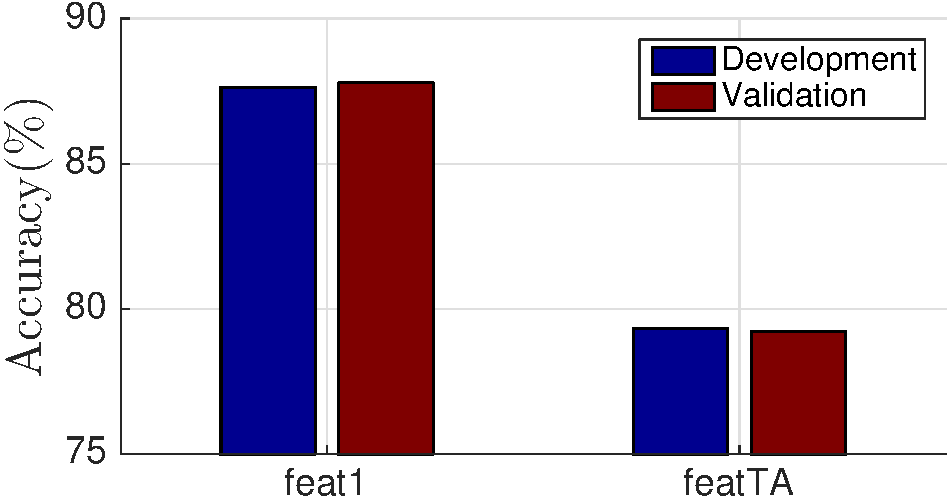
\includegraphics[width=60mm]{fig/feat.pdf}
\caption{Comparison between features}
\label{fig:feat}
\end{figure}

From Figure~\ref{fig:feat} we easily see significant improvement of \texttt{feat1} over \texttt{featTA}, proving our feature is superior and can help a lot in the following tasks.

\section{Algorithms}
\subsection{Linear Logistic Regression}
In the first model, we follow the principle of \emph{`linear first'}. We combine the \emph{Principal Component Analysis} (PCA)~\cite{jolliffe2002principal} and $L_2$-penalized logistic regression (LR). PCA is a well-known dimension reduction method, which seeks good representation of data with the criteria maximizing the variance. It� is an unsupervised learning method. To probe our problem, which we have some labeled data, we combine PCA with a supervised learning method, that is, linear logistic regression. The reason why we choose logistic regression is due to the requirement of track 1 which somewhat implies us to generate a `probability like' output. Another reason why we construct such model is efficiency. The feature set we generate is very high dimensional, and this will result in long training time.  PCA's dimension reduction makes the number of features used in logistic regression fewer. On the other hands, PCA find maximum variance data representation can be view as feature selection.

\subsubsection{Environment}
We implement such a pipeline model by Python using Scikit-learn~\cite{pedregosa2011scikit}.  

\subsubsection{Settings}
We use the absolute error for track 1 and 0/1 error for track 2 to train our model. We use grid search cross validation method to pick all parameters for our model such as the number of dimensions $N$ in PCA and $C$ in logistic regression formula below.
\begin{align*}
\min_{\w, c} \frac{1}{2}\w^\top\w + C \sum_n \log\para{\exp\para{-y_n\para{\w^\top\x + c}} + 1}
\end{align*}

The results of the grid search is reported below.

\begin{table}[!h]
\centering
\caption{The optimal parameters} 
\begin{tabular}{|M{0.15\linewidth}|M{0.35\linewidth}|M{0.35\linewidth}|}
\hline
& \texttt{featTA} & \texttt{feat1} \\ \hline
Track 1 & $N=31, C=10^{-1}$ & $N=122$, $C=10^2$ \\ \hline 
Track 2 & $N=10, C=10^{-4}$ & $N=185$, $C=10^4$ \\ \hline 
\end{tabular}
\end{table}

\subsubsection{Performance}
Before uploading to the online judge system, we evaluate the model with validation data. Track 1 is based upon 0/1 error, or $\eval^\01 = \sum_n \cond{\tilde y_n \neq y_n}$; and track 2 on absolute error, or $\eval^\abstxt = \sum_n \abs{\tilde y_n - y_n}$, where $\tilde y_n$ is the predicted class and $y_n$ is the ground truth. We then report the public score $S^\pub$ on the online judge system.

\begin{table}[!h]
\centering
\caption{$\eval$ and $S^\pub$ for logistic regression}
\begin{tabular}{|M{0.15\linewidth}|M{0.35\linewidth}|M{0.35\linewidth}|}
\hline
& \texttt{featTA} + LR & \texttt{feat1} + LR \\ \hline
Track 1 & $\eval^\abstxt=0.309$, $S_1^\pub=0.957$ & $\eval^\abstxt=0.290$, $S_1^\pub=0.960$ \\ \hline
Track 2 & $\eval^\01=0.155$, $S_2^\pub=0.837$ & $\eval^\01=0.152$, $S_2^\pub=0.856$ \\ \hline
\end{tabular}
\end{table}

Since we have yet to obtain satisfactory results, we decide to build a bootstrapped model with 100 small models of PCA and linear logistic regression. Each model is trained by using bootstrapped data with size equal to training set. The models are selected by 5 fold cross validation and a loose criteria that the $\eval^\01<0.17$ or $\eval^\abstxt<0.32$. The dimensionality of PCA is determined randomly between $\frac{D}{4}$ and $\frac{D}{2}$ where $D$ is the original dimensionality. The generation of small models is somewhat like the behavior of random forest. The performance of the improved bootstrapped LR (BS-LR) is shown below.

\begin{table}[!h]
\centering
\caption{$\eval$ and $S^\pub$ for BS-LR}
\begin{tabular}{|M{0.25\linewidth}|M{0.6\linewidth}|}
\hline
& \texttt{feat1} + BS-LR \\ \hline
Track 1 & $\eval^\abstxt=0.1839$, $S_1^\pub=0.9666$ \\ \hline
Track 2 & $\eval^\01=0.1220$, $S_2^\pub=0.8783$ \\ \hline
\end{tabular}
\end{table}

\subsection{\texttt{libsvm}~\cite{chang2011libsvm}}
Since we have tried linear models at the first sight and the results, yet not awful, do not look promising, we decide to empower the classifiers with kernels. That is, we try the performance with different kernel types in \texttt{libsvm}. However, we must keep in mind that using kernels entails potential overfitting problems, so we must keep an eye on both the development error and validation error. $\eval^\01$ is reported below.

\begin{table}[!h]
\centering
\caption{$\edev$ and $\eval$ for different kernels}
\begin{tabular}{|M{0.25\linewidth}|M{0.3\linewidth}|M{0.3\linewidth}|}
\hline
Kernel Type & $\edev^\01$ & $\eval^\01$ \\ \hline
Linear & $0.06 \sim 0.10$ & $0.30 \sim 0.40$ \\ \hline
Polynomial & $0.23$ & $0.30 \sim 0.35$ \\ \hline
Radial Basis Function & $0.15 \sim 0.20$ & $0.15 \sim 0.25$ \\ \hline  
\end{tabular}
\end{table}

It is obvious that radial basis function performs better than other kernel types. So we use it and keep adjusting parameters to improve. We only adjust parameters $\gamma$ and $C$ in C-SVM, because they improve the result more. The best $\eval^\01$ is 0.20 with parameters $\gamma=10^{-2}\sim10^{-1}$ and $C=10$. For regression, we use \texttt{libsvm} epsilon-SVR to train a single model. Using the model, we get the result below:

\begin{table}[!h]
\centering
\caption{$\eval$ and $S^\pub$ for \texttt{libsvm}}
\begin{tabular}{|M{0.25\linewidth}|M{0.6\linewidth}|}
\hline
& \texttt{feat1} + \texttt{libsvm} \\ \hline
Track 1 & $S_1^\pub=0.9329$ \\ \hline
Track 2 & $\eval^\01=0.20$, $S_2^\pub=0.8775$ \\ \hline
\end{tabular}
\end{table}

\subsection{Random Forest Regressor}
Classification and regression trees~\cite{lewis2000introduction} are known for their training efficiency, and, while the testing data exhibits similar distributions, evaluates fast with high accuracy. Having taught in class and implemented well by toolkits, we do not elaborate on how it is built here. 

\subsubsection{Environment}
The regression trees are implemented in Scikit-learn~\cite{pedregosa2011scikit} under Python.

\subsubsection{Settings}
We, in fact do not modify default settings for building a regression tree in Scikit-learn, because it internal uses $k$-fold cross-validation to avoid overfitting the data. Pruning the tree is implemented internally to remove unnecessary nodes. 
Since $\eval^\01$ for a single regression tree is only around $0.15$, we implement bootstrap on the regression tree, with a sample size of the original development set with replacement. 128 regression trees are aggregated to form a \emph{Random Forest Regressor} (RFR). 

\subsubsection{Performance}
We report the results of the random forest regressor here.

\begin{table}[!h]
\centering
\caption{$\eval$ and $S^\pub$ for RFR}
\begin{tabular}{|M{0.25\linewidth}|M{0.6\linewidth}|}
\hline
& \texttt{feat1} + RFR \\ \hline
Track 1 & $\eval^\abstxt=0.1926$, $S_1^\pub=0.9645$ \\ \hline
Track 2 & $\eval^\01=0.1226$, $S_2^\pub=0.8787$ \\ \hline
\end{tabular}
\end{table}

\subsection{Convolutional Neural Network}
There are many reasonable excuses for dropping a course, such as
\begin{itemize}
\item No interest on the first sight.
\item Having other courses of larger interests.
\item Having other personal issues which disallows his/her access to MOOC site.
\item Having obtained unsatisfactory marks and is unwilling to continue.
\end{itemize}
There are many other reasons, however, almost every single one of them need some more detailed information, or, \emph{time-related information}. In digital speech processing, we usually obtain 13-dimensional Mel-frequency cepstral coefficients, succeeded by first-order and second-order differentiations to obtain 39-dimensional coefficients. Similarly, if we have higher-order features, we may be able to predict with higher accuracy. To further exploit the time-relevant features such as \texttt{feat1.x2} and \texttt{feat.x3}, we resort to the recently popular \emph{Convolutional Neural Network}~(CNN)~\cite{lecun1989backpropagation}.

\subsubsection{Environment} 
Keras built on top of Tensorflow~\cite{abaditensorflow} is adopted to build the CNN. For efficiency, CUDA 7.5 toolbox is used, running on a NVidia GTX 980 Ti CPU. 

\subsubsection{Data pre-processing}
Training and testing feature vectors and feature maps are normalized together such that each dimension possesses a mean of zero a variance of unity.

\subsubsection{Settings}
We design the CNN considering the \texttt{GoogLeNet}~\cite{szegedy2014going} inception architecture. The abbreviations in the figure are:
\begin{itemize}
\item \texttt{FC}: \\ Fully connected layer followed by a dropout layer
\item \texttt{Conv (height}$\times$\texttt{width}$+$\texttt{stride}$/$\texttt{padding)}: \\ Convolutional layer 
\item \texttt{MaxPool (height}$\times$\texttt{width}$+$\texttt{stride}$/$\texttt{padding)}: \\ Max pooling layer
\item \texttt{Merge}: Merge inputs along depth
\end{itemize}

\begin{figure}[!h]
\centering
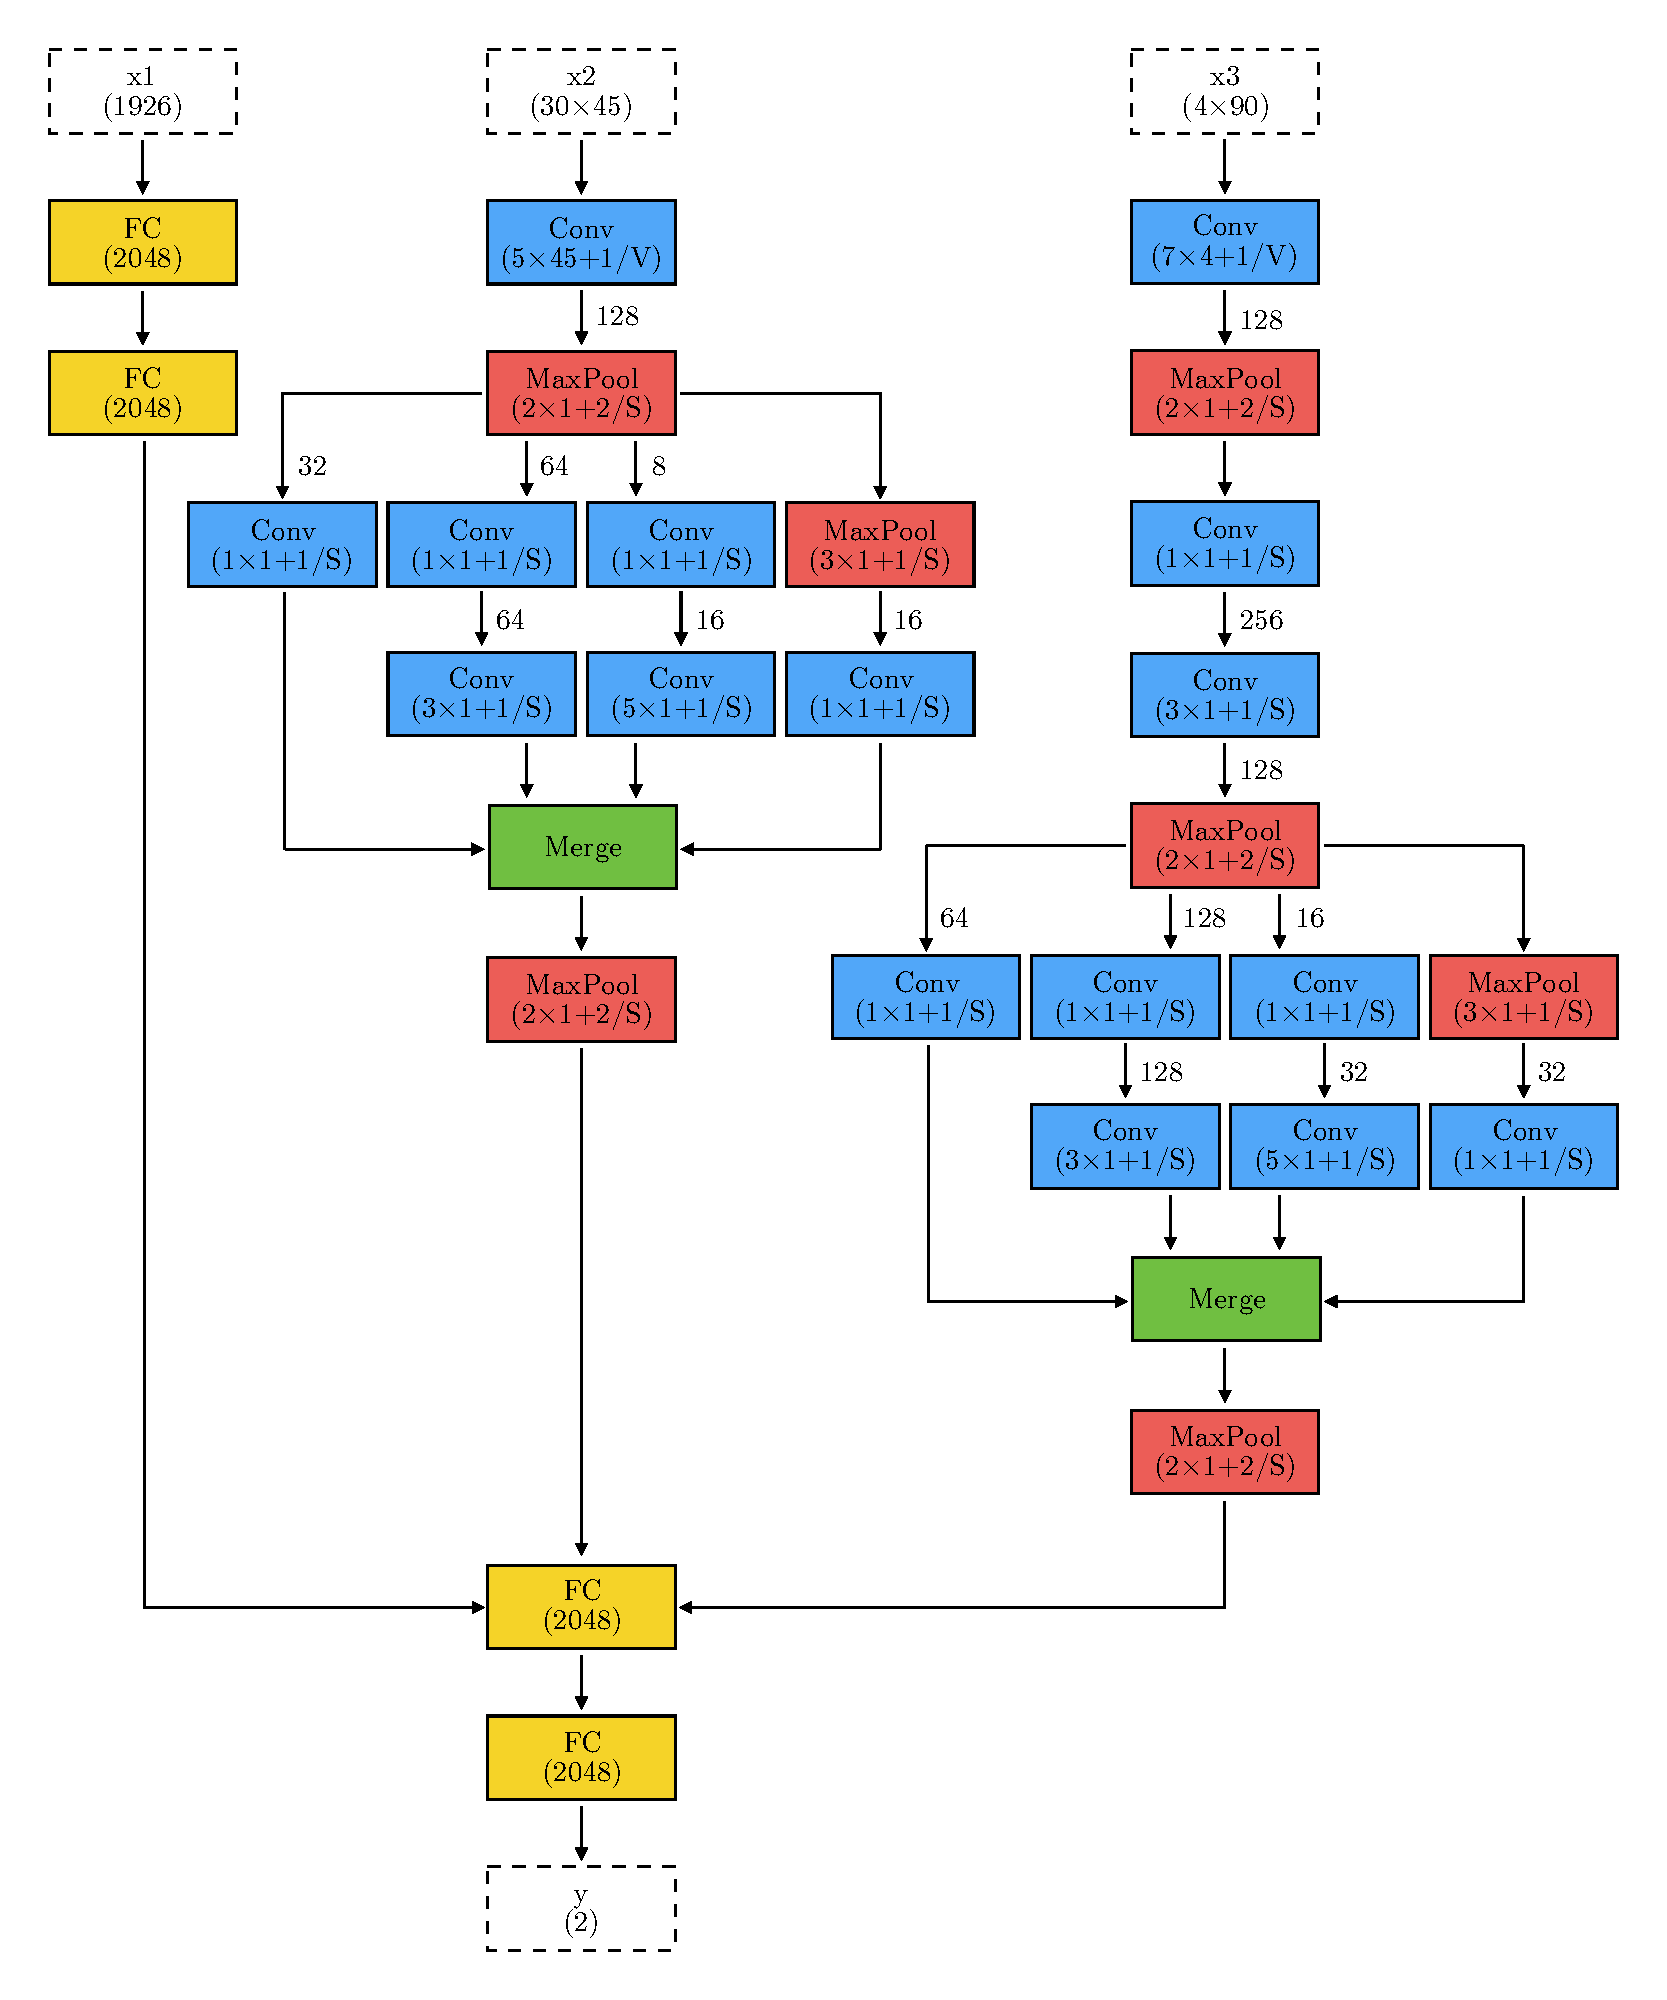
\includegraphics[width=\linewidth]{fig/cnn_graph.pdf}
\caption{CNN Architecture}
\label{fig:cnn_arch}
\end{figure}

After the neural network is built, we randomly initialize its weights, and then train with ADAM~\cite{kingma2014adam} optimizer under learning rate $10^{-5}$ over the development set. 

\subsubsection{Performance}
To determine how many epochs should be trained before stopping, we use the validation set error on the output. As we can see, the development loss drops steadily while the validation loss is already saturated after $3\sim 5$ epochs. Due to the limitation of the Keras toolbox, we are unable to evaluate the loss to a finer level, and by observing its verbose output, we know training for 5 epochs is enough.

\begin{figure}[!h]
\centering
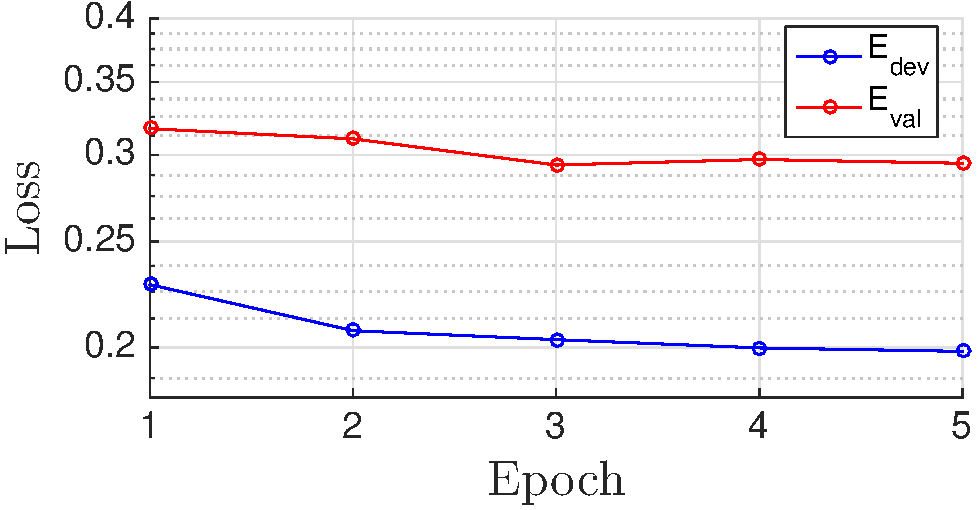
\includegraphics[width=80mm]{fig/cnn_val.pdf}
\caption{CNN training losses} 
\label{fig:cnn_val}
\end{figure}

Similarly, we evaluate $\eval^\01$ and $\eval^\abstxt$ for a single CNN model and report its public score $S^\pub$.

\begin{table}[!h]
\centering
\caption{$\eval$ and $S^\pub$ for CNN}
\begin{tabular}{|M{0.25\linewidth}|M{0.6\linewidth}|}
\hline
& \texttt{feat1} + CNN \\ \hline
Track 1 & $\eval^\abstxt=0.1904$, $S_1^\pub=0.9686$ \\ \hline
Track 2 & $\eval^\01=0.1120$, $S_2^\pub=0.8847$ \\ \hline
\end{tabular}
\end{table}

\subsection{Comparison}
SVM does not perform well under these settings. Comparing these models, combination of PCA and logistic regression is a linear model and the output from logistic regression gives some physical meaning of probability. The linear model gives the interpretability but cannot calibrate non-linear behavior, making its performance limited.

\begin{table}[!h]
\scriptsize
\centering
\caption{A comparison between methods}
\begin{tabular}{|M{0.25\linewidth}|*3{M{0.17\linewidth}|}}
\hline
& BS-LR & RFR & CNN \\ \hline
Efficiency 
& \FiveStar\FiveStar\FiveStar\FiveStar\FiveStar 
& \FiveStar\FiveStar\FiveStar\FiveStarOpen\FiveStarOpen
& \FiveStar\FiveStarOpen\FiveStarOpen\FiveStarOpen\FiveStarOpen \\ \hline
Scalability 
& \FiveStar\FiveStar\FiveStarOpen\FiveStarOpen\FiveStarOpen
& \FiveStar\FiveStar\FiveStar\FiveStar\FiveStarOpen
& \FiveStar\FiveStar\FiveStar\FiveStar\FiveStar \\ \hline
Popularity
& \FiveStar\FiveStar\FiveStar\FiveStarOpen\FiveStarOpen
& \FiveStar\FiveStar\FiveStar\FiveStarOpen\FiveStarOpen
& \FiveStar\FiveStar\FiveStar\FiveStar\FiveStar \\ \hline
Interpretability
& \FiveStar\FiveStar\FiveStar\FiveStarOpen\FiveStarOpen
& \FiveStar\FiveStar\FiveStar\FiveStar\FiveStarOpen
& \FiveStar\FiveStarOpen\FiveStarOpen\FiveStarOpen\FiveStarOpen \\ \hline
Performance
& \FiveStar\FiveStar\FiveStarOpen\FiveStarOpen\FiveStarOpen
& \FiveStar\FiveStar\FiveStar\FiveStarOpen\FiveStarOpen
& \FiveStar\FiveStar\FiveStar\FiveStar\FiveStar \\ \hline
Track 1 $S_1^\pub$
& 0.9666
& 0.9645
& 0.9686 \\ \hline
Track 2 $S_2^\pub$
& 0.8783
& 0.8787
& 0.8847 \\ \hline
\end{tabular}
\end{table}

\section{Model Blending}
Over the mere several days we, in total have trained 73 bootstrapped logistic regression (BS-LR) models, 29 random forest regressors (RFR), and 81 convolutional neural networks (CNN). 

In the beginning, we try to use uniform blending to aggregate models using the average predictions of the models as the blending result. Then we try to use linear blending. Using validation accuracy as the weight, we calculate the mean of all models. If the mean is more than 0.5, then the prediction is 1 otherwise 0.
However, the uniform blending and linear blending do not improve the result much, because the predictions of every model are too similar. Then the final blending result is almost equal to the best result.

\subsection{Settings}
Finally we resort to \emph{neural network blending}, that is, we train a small neural network on top of the prediction results from 183 models. The model built is a mere $183-128-2$ network with \texttt{tanh} activation units, with a learning rate of $10^{-3}$, allowing soft and gentle training. In fact, we use half the validation data for blending model training, and half the validation data for blending model validation. Instead of using stochastic gradient descent, we use the whole training validation data for gradient calculation.

\begin{figure}[!h]
\centering
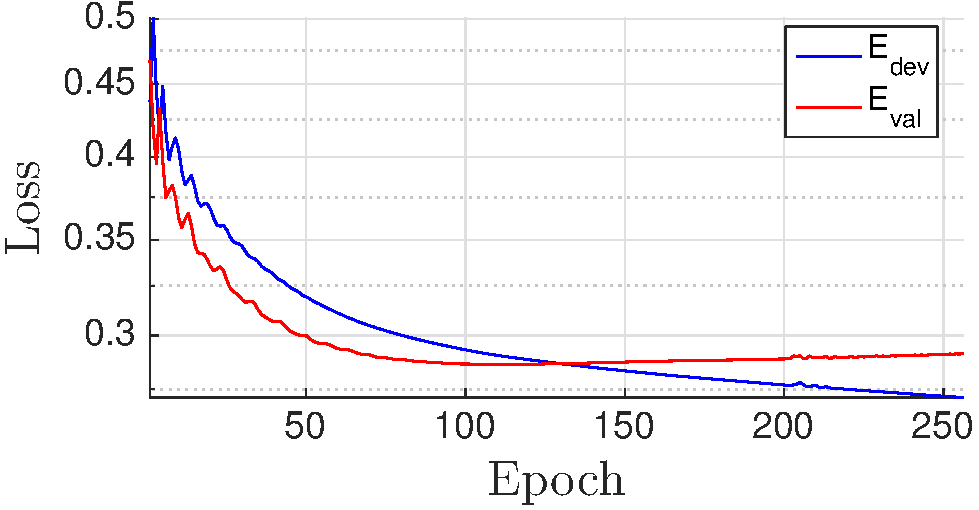
\includegraphics[width=80mm]{fig/blend_val.pdf}
\caption{Blending training losses} 
\end{figure}

\subsection{Performance}
To determine how many epochs should be trained before stopping, we use the validation set error on the output. As we can see, the development loss drops steadily while the validation loss is already rising at 100 epochs. We decide to train the blending model with all the validation data for 64 epochs at last, which is the half of 128, since we only had half the data at blending model validation. In the end we are able to achieve a better result.

\begin{table}[!h]
\centering
\caption{$\eval$ and $S^\pub$ for Blending model}
\begin{tabular}{|M{0.25\linewidth}|M{0.6\linewidth}|}
\hline
& \texttt{feat1} + Blend \\ \hline
Track 1 & $\eval^\abstxt=0.1712$, $S_1^\pub=0.9703$ \\ \hline
Track 2 & $\eval^\01=0.1084$, $S_2^\pub=0.8879$ \\ \hline
\end{tabular}
\end{table}

\section{Conclusion}
Finally we are able to achieve a score of $S_1^\pub=0.9703$ and $S_2^\pub=0.8879$ despite the fact that we did not specifically optimize for neither tracks according to their measures. What we can do is we pair the samples and, if they have different ground truths, we maximize their margins, and in this way the results for track 1 can be optimized. On the other hand, we can reweight the samples in track 2 according to the inverse of courses taken to emphasize on people with lesses courses. While regression methods are generally better for track 1 and classification methods are for track 2, we only took regression methods for both tracks, and that may degrade our result a little. At the end, for the neural network blending, we can train a large ensemble of small neural networks and make them collaborate to give a better final result.

\section{Division of Work}
\begin{itemize}
\item Tzu-Ming Harry Hsu (B00901168): Feature engineering, RFR, CNN, NN blending, and report compilation
\item Yi Hsiao (R04945027): Feature engineering, and PCA/LR
\item Li-Yuan Liu (R04944018): Feature engineering, \texttt{libsvm}, and linear blending
\end{itemize}

\bibliographystyle{ieeetr}
\bibliography{bib}

\end{document}
